\begin{align*}
g(\alpha) &= \min\limits_x L(x,\alpha) \\
&= \min\limits_x (f_0(x) + \sum\limits_{i=0}^{m} \alpha_i f_i(x)) \\
\Rightarrow g(\alpha) &= \min\limits_x ( f_0(x) + \alpha_1 f_1(x) ) \\
&= f_0(x^*) + \alpha_1 f_1(x^*)
\end{align*}

Since $f_0(x)$ and $f_1(x)$ are convex, and furthermore $\alpha$ is positive or 0, the minimized expression is convex and has exactly one minimum. This minimum has to be global.

\begin{align*}
0 &= \frac{\di}{\di x} ( f_0(x) + \alpha_1 f_1(x) ) \\
  &= f_0'(x) + \alpha f_1'(x) \\
  &= 2x + \alpha_1 ( x-4 + x-2 ) \\
  &= x (2+2 \alpha_1) - 6 \alpha_1 \\
  \Rightarrow x^* &= \frac{3 \alpha_1}{1+\alpha_1}
\end{align*}

\[ g(\alpha) = f_0(\frac{3 \alpha_1}{1+\alpha_1}) + \alpha_1 f_1(\frac{3 \alpha_1}{1+\alpha_1}) \]

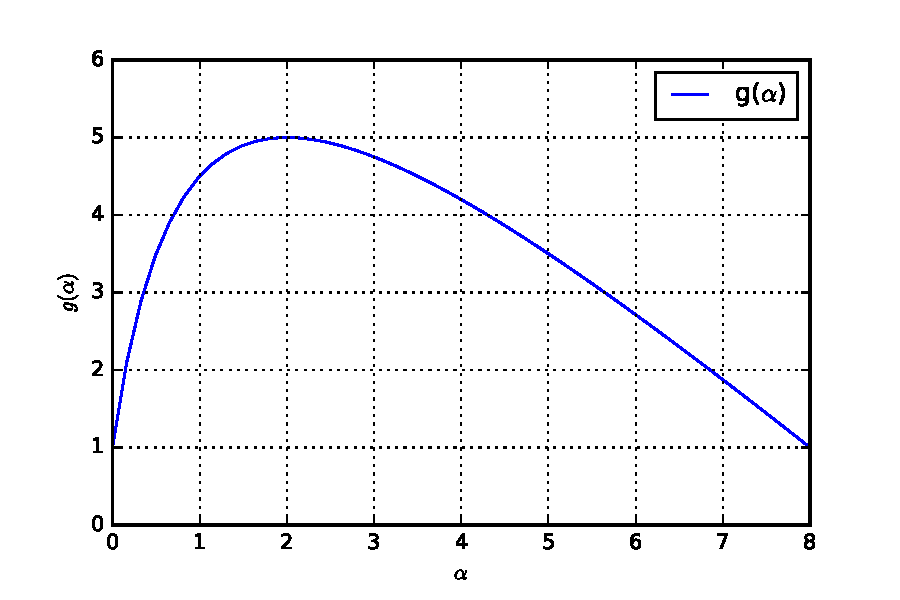
\includegraphics[scale=0.7]{problems/code/prob7_fig.pdf}

